%%%%%%%%%%%%%%%% Springer %%%%%%%%%%%%%%%%%%%%%%%%%%%%%%%%%%
% RECOMMENDED %%%%%%%%%%%%%%%%%%%%%%%%%%%%%%%%%%%%%%%%%%%%%%%%%%%
\documentclass[graybox]{svmult}
% choose options for [] as required from the list
% in the Reference Guide
\usepackage{type1cm}        % activate if the above 3 fonts are
                            % not available on your system
%
\usepackage{makeidx}         % allows index generation
%\usepackage{graphicx}        % standard LaTeX graphics tool
                             % when including Fig.~files
\usepackage{multicol}        % used for the two-column index
\usepackage[bottom]{footmisc}% places footnotes at page bottom
\usepackage{newtxtext}       % 
\usepackage{newtxmath}       % selects Times Roman as basic font
% see the list of further useful packages
% in the Reference Guide
%\makeindex             % used for the subject index
                       % please use the style svind.ist with
                       % your makeindex program
%%%%%%%%%%%%%%%%%%%%%%%%%%%%%%%%%%%%%%%%%%%%%%%%%%%%%%%%%%%%%%%%%%%%%%%%%%%%%%%%%%%%%%%%%
% \usepackage{amsmath}
% \usepackage{ascmac}
\usepackage[dvipdfmx]{graphicx}  % for EPS and PDF 
% \usepackage{url}
\usepackage{fancyvrb}
% \usepackage{makeidx}
% \usepackage{float}
% \usepackage[dvipdfmx]{color}
% \usepackage{ulem}
% \usepackage[switch*,pagewise]{lineno}
% \usepackage[dvipdfm,bookmarkstype=toc,urlcolor=black,%
%     linkcolor=black,citecolor=black,bookmarks=false]{hyperref}
% \usepackage{fancyhdr}

\usepackage{listings}
\lstset{%
 language={C},
% basicstyle={\scriptsize},%
% identifierstyle={\scriptsize},%
 basicstyle={\small},%
 identifierstyle={\small},%
% commentstyle={\small\itshape},%
%commentstyle={\scriptsize},%
commentstyle={\small},%
 keywordstyle={\small\bfseries},%
 ndkeywordstyle={\small},%
stringstyle={\small\ttfamily},
 frame={tb},
 breaklines=true,
 columns=[l]{fullflexible},%
 numbers=left,%
 xrightmargin=1zw,%
 xleftmargin=1.5zw,%
 numberstyle={\small},%
 stepnumber=1,
 numbersep=1zw,%
% lineskip=-0.1ex%
}

\def\|{\verb|}

%\newenvironment{myfigure}{\begin{figure}[ht]\begin{center}}{\end{center}\end{figure}}

\def\Directive#1{{\tt #1}\index{#1@{\tt #1}}\index{Directive!#1@{\tt #1}}}

%\def\Syntax#1{\index{{\tt #1}}\index{Syntax!{\tt #1}}}
\def\Syntax#1{\index{Syntax!#1@{\tt #1}}}

\def\Term#1{{#1}\index{#1}}

%\def\Example#1{\index{#1}\index{Example!{\tt #1}}}
\def\Example#1{\index{Example!#1@{\tt #1}}}

\def\Intrinsic#1{\index{#1@{\tt #1}}\index{Intrinsic and Library Procedures!#1@{\tt #1}}}

\DefineVerbatimEnvironment{Fexample}{Verbatim}{numbers=left,numbersep=3pt,stepnumber=5,%
frame=single,label=\Fort}
\DefineVerbatimEnvironment{FexampleR}{Verbatim}{numbers=right,numbersep=3pt,stepnumber=5,%
frame=single,label=\Fort}

\DefineVerbatimEnvironment{Cexample}{Verbatim}{numbers=left,numbersep=3pt,stepnumber=5,%
frame=single,label=\C}
\DefineVerbatimEnvironment{CexampleR}{Verbatim}{numbers=right,numbersep=3pt,stepnumber=5,%
frame=single,label=\C}

\DefineVerbatimEnvironment{XFexample}{Verbatim}{numbers=left,numbersep=3pt,stepnumber=5,%
frame=single,label=\XMPF}
\DefineVerbatimEnvironment{XFexampleR}{Verbatim}{numbers=right,numbersep=3pt,stepnumber=5,%
frame=single,label=\XMPF}

\DefineVerbatimEnvironment{XCexample}{Verbatim}{numbers=left,numbersep=3pt,stepnumber=5,%
frame=single,label=\XMPC}
\DefineVerbatimEnvironment{XCexampleR}{Verbatim}{numbers=right,numbersep=3pt,stepnumber=5,%
frame=single,label=\XMPC}

\DefineVerbatimEnvironment{MPICexample}{Verbatim}{numbers=right,numbersep=3pt,stepnumber=5,%
frame=single,label=MPI C}
\DefineVerbatimEnvironment{MPIFexample}{Verbatim}{numbers=right,numbersep=3pt,stepnumber=5,%
frame=single,label=MPI Fortran}


\setcounter{secnumdepth}{4}
\setcounter{tocdepth}{3}
\setcounter{totalnumber}{6}
\usepackage{fancyhdr}

\let\olditemize\itemize
\renewcommand{\itemize}{
   \olditemize
   \setlength{\itemsep}{8pt}
   \setlength{\parskip}{0pt}
   \setlength{\parsep}{0pt}
}

% \parindent = 0pt
% \hoffset=0cm
% \oddsidemargin=0cm
% \evensidemargin=0cm
% \textwidth=16cm
% \topmargin=-1cm
% \voffset=0cm
% \textheight=24cm

\def\progenv{\baselineskip=10pt\tt\progspecial{`}\parindent=0.3cm}
\def\shellenv{\baselineskip=10pt\tt\progspecial{`}\parindent=0.3cm\nolineno}

\renewcommand{\topfraction}{.99}
\renewcommand{\bottomfraction}{.99}

\def\openb{{\it [}}
\def\closeb{{\it ]}}
\def\XMP{XcalableMP}
\def\XACC{XcalableACC}
\def\OACC{OpenACC}
\def\OMP{OpenMP}
\def\XMPF{XcalableMP Fortran}
\def\XMPC{XcalableMP C}
\def\XACCF{XcalableACC Fortran}
\def\XACCC{XcalableACC C}
\def\Syntax#1{\index{Syntax!#1@{\tt #1}}}
\def\Example#1{\index{Example!#1@{\tt #1}}}
%
\def\phrule{\vspace{0.2cm}\hrule\vspace{0.05cm}\hrule}
\def\qhrule{\vspace{0.2cm}\hrule}
\def\dhrule{\hrule\vspace{0.05cm}\hrule}
\def\bsquare{\rule[-2pt]{5pt}{10pt}}
%
\newenvironment{mytable}[3]{\begin{table}[ht]\caption{#1}\label{#2}\vspace*{-0.3cm}\begin{center}\begin{tabular}{#3}}{\end{tabular}\end{center}\end{table}}
\newenvironment{myfigure}{\begin{figure}[ht]\begin{center}}{\end{center}\end{figure}}
%
\DefineVerbatimEnvironment{XACCFexampleL}{Verbatim}{numbers=left,numbersep=3pt,stepnumber=5,frame=single,label=\XACCF}
\DefineVerbatimEnvironment{XACCCexampleR}{Verbatim}{numbers=right,numbersep=3pt,stepnumber=5,frame=single,label=\XACCC}
\DefineVerbatimEnvironment{XACCCexampleL}{Verbatim}{numbers=left,numbersep=3pt,stepnumber=5,frame=single,label=\XACCC}

%%%%%%%%%%%%%%%%%%%%%%%%%%%%%%%%%%%%%%%%%%%%%%%%%%%%%%%%%%%%%%%%%%%%%%%%%%%%%%%%%%%%%%%%%

% my definitions
\newcommand{\requirement}{{\bf Requirement to the compiler.} }
\newcommand{\fig}[1]{Figure~\ref{fig:#1}}
\newcommand{\tab}[1]{Table~\ref{tab:#1}}


%%%%%%%%%%%%%%%%%%%%%%%%%%%%%%%%%%%%%%%%%%%%%%%%%%%%%%%%%%%%%%%%%%%%%%%%%%%%%%%%%%%%%%%%%


\begin{document}



\title*{Coarrays in the Context of XcalableMP}
% Use \titlerunning{Short Title} for an abbreviated version of
% your contribution title if the original one is too long

\author{H.\ Iwashita and M.\ Nakao}
% Use \authorrunning{Short Title} for an abbreviated version of
% your contribution title if the original one is too long

\institute{
Hidetoshi Iwashita 
\at Fujitsu Limited, 140 Miyamoto, Numazu-shi, Shizuoka 410-0396, Japan,
\email{iwashita.hideto@fujitsu.com}
\and
Masahiro Nakao \at RIKEN Center for Computational Science,
7-1-26 Minatojima-minami-machi, Chuo-ku, Kobe, Hyogo 650-0047, Japan,
\email{masahiro.nakao@riken.jp}
}

%
% Use the package "url.sty" to avoid
% problems with special characters
% used in your e-mail or web address
%
\maketitle

\abstract{@@@ XcalableACC (XACC) is an extension of XcalableMP for
accelerated clusters. It is defined as a diagonal integration of
XcalableMP and OpenACC, which is another directive-based language
designed to program heterogeneous CPU/accelerator systems. XACC has
features for handling distributed-memory parallelism, inherited from
XMP, offloading tasks to accelerators, inherited from OpenACC, and
two additional functions: data/work mapping among multiple accelerators
and direct communication between accelerators.
}

%\tableofcontents
\clearpage

%
% Sections
%

\section{Introduction}\label{chap:intro}

\pagenumbering{arabic}
\setcounter{page}{1}

This document defines the specification of {\XACC} (XACC) which is an extension
of {\XMP} version 1.3\cite{xmp} and {\OACC} version 2.5\cite{openacc}.
{\XACC} provides a parallel programming model for accelerated clusters
which are distributed memory systems equipped with accelerators.

In this document,
terminologies of {\XMP} and {\OACC} are indicated by {\bf bold font}.
For details, refer to each specification\cite{xmp,openacc}.

The works on XACC and the Omni XcalableACC compiler was
supported by the Japan Science and Technology Agency, 
Core Research for Evolutional Science and Technology program entitled 
``Research and Development on Unified Environment of Accelerated
Computing and Interconnection for Post-Petascale Era'' in the research
area of ``Development of System Software Technologies for Post-Peta
Scale High Performance Computing.''

\subsection{Hardware Model}
The target of {\XACC} is an accelerated cluster,
a hardware model of which is shown in Fig. \ref{fig:hardware}.

\begin{myfigure}
  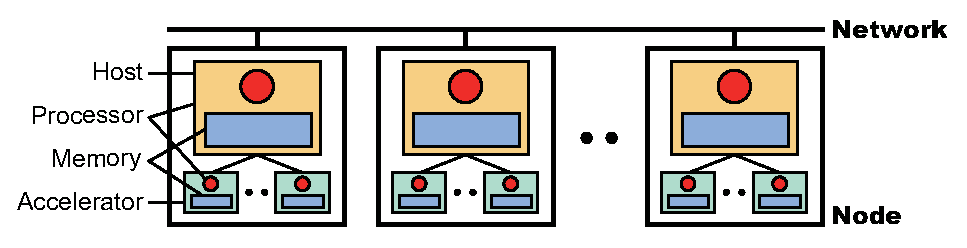
\includegraphics[width=\textwidth]{figs/hardware.eps}
  \caption{Hardware Model}\label{fig:hardware}
\end{myfigure}

An execution unit is called {\bf node} as with {\XMP}.
Each {\bf node} consists of a single host and multiple accelerators (such as GPUs and Intel MICs).
Each host has a processor, which may have several cores, and own local memory.
Each accelerator also has them.
Each {\bf node} is connected with each other via network.
Each {\bf node} can access its local memories directly and remote memories,
that is, the memories of another {\bf node} indirectly.
In a host,
the accelerator memory may be physically and/or virtually separate from the host memory as with the memory model of {\OACC}.
Thus,
a host may not be able to read or write the accelerator memory directly.

\subsection{Programming Model}
{\XACC} is a directive-based language extension based on Fortran 90 and ISO C90 (ANSI C90).
To develop applications on accelerated clusters with ease,
{\XACC} extends {\XMP} and {\OACC} independently as follow:
(1) {\XMP} extensions are to facilitate cooperation between {\XMP} and {\OACC} directives.
(2) {\OACC} extensions are to deal with multiple accelerators.

\subsubsection{{\XMP} Extensions}
In a program using the {\XMP} extensions,
{\XMP}, {\OACC}, and {\XACC} directives are used.
Fig. \ref{fig:concept} shows a concept of the {\XMP} extensions.

\begin{myfigure}
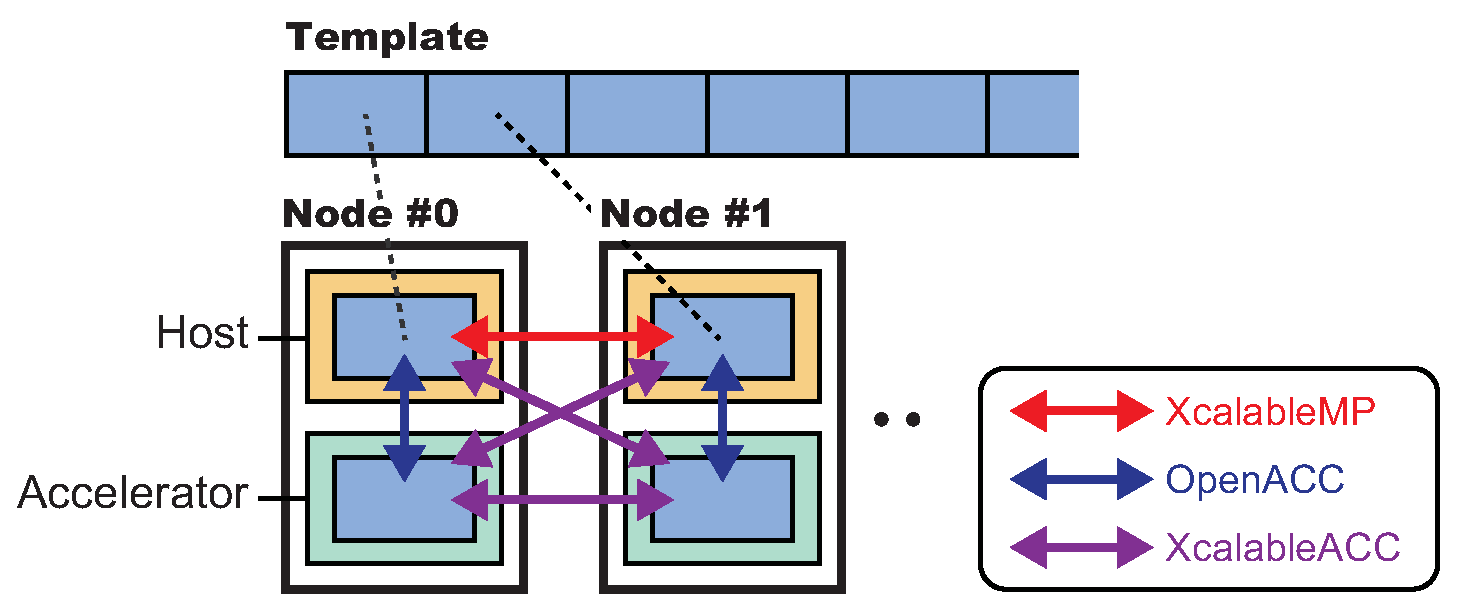
\includegraphics[width=\textwidth]{figs/concept.eps}
  \caption{Concept of {\XMP} Extensions}\label{fig:concept}
\end{myfigure}

{\XMP} directives define a {\bf template} and a {\bf node set}.
The {\bf template} represents a global index space, which is distributed onto the {\bf node set}.
Moreover, {\XMP} directives declare {\bf distributed arrays},
parallelize loop statements and transfer data among host memories according to the distributed {\bf template}.
{\OACC} directives transfer the {\bf distributed arrays} between host memory and accelerator memory on the same {\bf node}
and execute the loop statements parallelized by {\XMP} on accelerators in parallel.
{\XACC} directives, which are {\XMP} communication directives with an {\tt acc} clause, 
transfer data among accelerator memories and between accelerator memory and host memory on different {\bf nodes}.
Moreover, 
{\bf coarray} features also transfer data on different nodes.

%The {\XMP} extension is defined to develop parallel applications with keeping the sequential code image.
Note that 
the {\XMP} extensions are not a simple combination of {\XMP} and {\OACC}.
For example, 
if you represent communication of {\bf distributed array} among accelerators shown in Fig. \ref{fig:concept} by the combination of {\XMP} and {\OACC},
you need to specify explicitly communication between host and accelerator by {\OACC} and that between hosts by {\XMP}.
Moreover,
you need to calculate manually indices of the {\bf distributed array} owned by each {\bf node}.
By contrast,
{\XACC} directives can represent such communication among accelerators directly using global indices.

\subsubsection{{\OACC} Extensions}
The {\OACC} extension can represent offloading works and data to multiple-accelerators on a {\bf node}.
Fig. \ref{fig:concept_acc_ex} shows a concept of the {\OACC} extension.

\begin{myfigure}
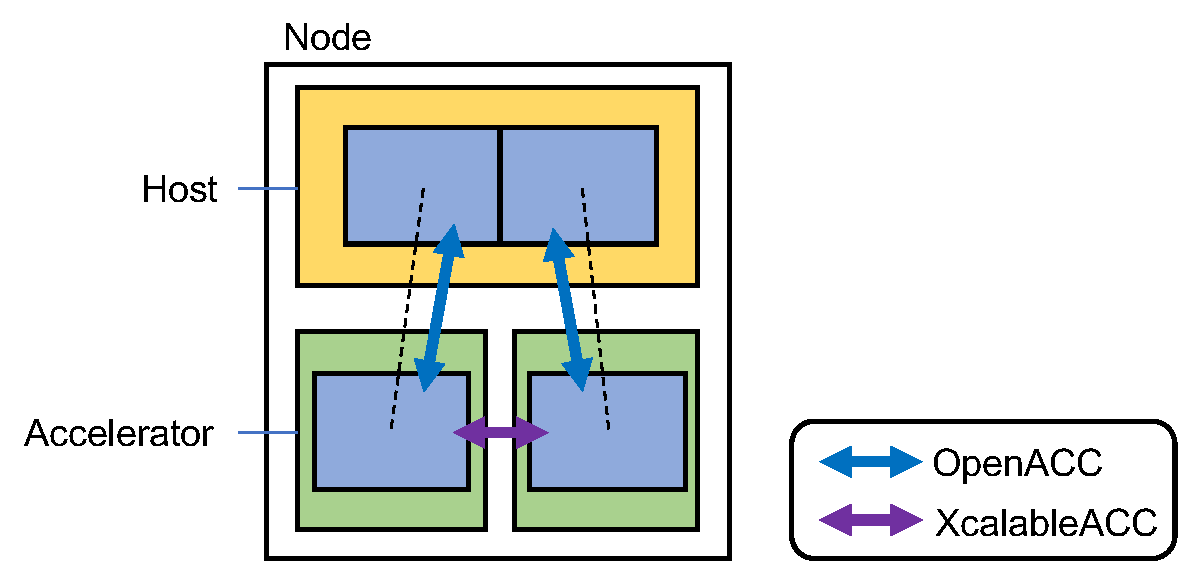
\includegraphics[width=\textwidth]{figs/concept_acc_ext.pdf}
  \caption{Concept of {\OACC} Extension}\label{fig:concept_acc_ex}
\end{myfigure}

{\OACC} extension directive defines a {\bf device set}.
The {\bf device set} represents a set of devices on a {\bf node}.
Futher, {\OACC} extension directives declare {\bf distributed arrays} on the {\bf device set} while maintaining the arrays on the host memory, and the directives distribute offloading loop statement and memory copy between host and device memories for the {\bf distributed-arrays}.
Moreover, {\OACC} extension directives synchronizes devices among the {\bf device set}.
{\XACC} directives also transfer data between device memories on the {\bf node}.

\subsection{Execution Model}
The execution model of {\XACC} is a combination of those of {\XMP} and {\OACC}.
While the execution model of a host CPU programming is based on that of {\XMP},
that of an accelerator programming is based on that of {\OACC}.
Unless otherwise specified,
each {\bf node} behaves exactly as specified in the {\XMP} specification\cite{xmp} or the {\OACC} specification\cite{openacc}.
%For details, refer to each specification\cite{xmp,openacc}.

An {\XACC} program execution is based on the SPMD model, 
where each {\bf node} starts execution from the same main routine and keeps executing the same code independently (i.e. asynchronously), 
which is referred to as the replicated execution
until it encounters an {\XMP} construct or an {\XMP}-extension construct.
In particular,
the {\XMP}-extension construct may allocate, deallocate, or transfer data on accelerators.
An {\OACC} construct or an {\OACC}-extension construct may define {\bf parallel regions}, such as work-sharing loops, 
and offloads it to accelerators under control of the host.

When a {\bf node} encounters a loop construct 
targeted by a combination of {\XMP} {\tt loop} and {\OACC} {\tt loop} directives,
it executes the loop construct in parallel with other {\bf accelerators},
so that each iteration of the loop construct is independently executed by the {\bf accelerator}
where a specified data element resides.

When a {\bf node} encounters a {\XACC} synchronization or a {\XACC} communication directive,
synchronization or communication occurs between it and other accelerators.
That is, such {\bf global constructs} are performed collectively by the {\bf current executing nodes}.
Note that neither synchronizations nor communications occur without these constructs specified.

\subsection{Data Model}
There are two classes of data in {\XACC}: {\bf global data} and {\bf local data} as with {\XMP}. 
Data declared in an {\XACC} program are local by default.
Both {\bf global data} and {\bf local data} can exist on host memory and accelerator memory.
About the data models of host memory and accelerator memory, refer to the OpenACC specification\cite{openacc}.

{\bf Global data} are ones that are distributed onto the {\bf executing node set} by the {\tt align} directive.
Each fragment of a {\bf global data} is allocated in host memory of a {\bf node} in the {\bf executing node set}.
{\OACC} directives can transfer the fragment from host memory to accelerator memory.

{\bf Local data} are all of the ones that are not global.
They are replicated in the local memory of each of the {\bf executing nodes}.

A {\bf node} can access directly only {\bf local data} and sections of {\bf global data} that are allocated in its local memory.
To access data in remote memory, 
explicit communication must be specified in such ways as the global communication constructs and the {\bf coarray} assignments.

Particularly in {\XACCF}, 
for common blocks that include any global variables, 
the ways how the storage sequence of them is defined and how the storage association of them is resolved are implementation-dependent.

% \subsection{Directive Format}
% This section describes the syntax and behavior of {\XMP} and {\OACC} directives in {\XACC}.
% In this document, 
% the following notation is used to describe the directives.

% \vspace{0.5cm}%
% \begin{tabular}{ll}
% {\tt xxx} & {\tt type-face} characters are used to indicate literal type characters. \\
% {\it xxx...} & If the line is followed by ``...'', then xxx can be repeated. \\
% {\it [xxx]} & {\it xxx} is optional. \\
% {\bsquare} & The syntax rule continues. \\
% \verb![F]! & The following lines are effective only in {\XACCF}. \\
% \verb![C]! & The following lines are effective only in {\XACCC}. \\
% \end{tabular}
% \vspace{0.5cm}%

% In {\XACCF}, 
% {\XMP} and {\OACC} directives are specified using special comments that are identified by unique sentinels {\tt\verb|!$xmp|} and {\tt\verb|!$acc|} respectively.
% the directives follow the rules for comment lines of either the Fortran free or fixed source form,
% depending on the source form of the surrounding program unit\footnote{Consequently, the rules of comment lines that an
% {\XMP} directive follows is the same as the ones that an {\OMP} directive follows.}.
% The directives are case-insensitive.

% \vspace{0.5cm}
% \Syntax{directive}
% \begin{tabular}{ll}
% \verb![F]! & \verb|!$xmp| {\it directive-name clause} \\
% \verb![F]! & \verb|!$acc| {\it directive-name clause} \\
% \end{tabular}
% \vspace{0.5cm}

% In {\XACC}, 
% {\XMP} and {\OACC} directives are specified using the \verb|#pragma| mechanism provided by the C standards.
% the directives are case-sensitive.

% \vspace{0.5cm}
% \Syntax{directive}
% \begin{tabular}{ll}
% \verb![C]! & \verb|#pragma xmp| {\it directive-name clause} \\
% \verb![C]! & \verb|#pragma acc| {\it directive-name clause} \\
% \end{tabular}
% \vspace{0.5cm}

%Directives are classified as {\bf declarative directives} and {\bf executable directives}\cite{xmp}.
%
%The {\bf declarative directives} are {\tt nodes}, {\tt template}, {\tt distribute}, {\tt align},
%{\tt shadow}, {\tt coarray}, {\tt declare}, and {\tt routine} directives.
%
%The {\bf executable directives} are {\tt template\_fix}, {\tt task}, {\tt tasks}, {\XMP} {\tt loop}, 
%{\tt array}, {\tt reflect}, {\tt reflect\_init}, {\tt reflect\_do}, {\tt gmove}, {\tt barrier}, 
%{\tt reduction}, {\tt bcast}, {\tt wait\_async},
%{\tt parallel}, {\tt kernels}, {\tt data}, {\tt host\_data}, {\OACC} {\tt loop},
%{\tt cache}, {\tt atomic}, {\tt init}, {\tt shutdown}, {\tt set}, {\tt update}, 
%{\tt wait}, {\tt enter\_data}, and {\tt exit\_data} directives.
%An {\bf executable directive} and its associated user code make up an {\XACC} construct, 
%as in the following format:
%
%\vspace{0.5cm}
%\begin{tabular}{ll}
%\verb![F]! & \verb|!$xmp| {\it directive-name clause} ...\\
% & \hspace{0.5cm} {\it structured-block} \\
%\verb![F]! & \verb|!$acc| {\it directive-name clause} ...\\
% & \hspace{0.5cm} {\it structured-block} \\
%\end{tabular}
%
%\vspace{0.3cm}
%
%\begin{tabular}{ll}
%\verb![C]! & \verb|#pragma xmp| {\it directive-name clause} ...\\
% & \hspace{0.5cm} {\it structured-block} \\
%\verb![C]! & \verb|#pragma acc| {\it directive-name clause} ...\\
% & \hspace{0.5cm} {\it structured-block} \\
%\end{tabular}
%\vspace{0.5cm}

% \subsection{Organization of This Document}
% The remainder of this document is structured as follows:

% \begin{itemize}
%  \item Chapter 2: {\XMP} Extensions
%  \item Chapter 3: {\OACC} Extensions
% \end{itemize}
 
%\cleardoublepage

\section{Coarray Features and the Key of the Implementation}\label{sec:lang}

XMP Fortran language specification supports a major part of coarray features defined in 
Fortran~2008 standard~\cite{F08}, and intrinsic procedures 
{\tt CO\_SUM}, {\tt CO\_MAX}, {\tt CO\_MIN} and {\tt CO\_BROADCAST} defined in 
Fortran~2018 standard~\cite{F18} were supported.
And also XMP C language specification extended to support coarray features.

This section introduces the coarray features and what is required
to the compiler in order to implement the coarray features.


%-----------------------------------------------------------------------------
\subsection{Images Mapped to XMP Nodes}
%-----------------------------------------------------------------------------

In the Fortran standard, an {\bf image} is defined as a instance of a program. 
Each image executes the same program and has its own data individually 
(SPMD: Single Program/Multiple Data).
Each image has a different image index, which is one of $1, \cdots, n$, 
where $n$ is the number of images. 
While Fortran standard does not specify actually where each image is executed, 
XMP defines that the images are mapped in tern to the executing nodes. 
Therefore, image $k$ is always executed simply on executing node $k$, 
where $1 \leq k \leq n$ and 
$n$ is the number of images and also the number of the executing nodes. 

Note that the executing nodes can be a subset of the entire (initial) node set. 
For example, two distinct node sets can execute two coarray subprograms concurrently.
When the execution encounters a {\tt TASK} directive specified with a subset of nodes,
the corresponding subset of the images will be the executing images for the
TASK region. 
The number of images and my image number, which are given by inquire functions
{\tt num\_images} and {\tt this\_image}, also match with the executing images, and
the {\tt SYNC\_IMAGES} statement synchronizes among the executing images.
When the execution encounters the {\tt END TASK} directive corresponding to the
{\tt TASK} directive, the set of executing image is reinstated.
Unless the {\tt TASK} and {\tt END TASK} directives are used, coarray features are 
compatible to the ones of the Fortran standard. 

%   Coarray features can be used inside the TASK directive blocks. As default,
%   each coarray image is mapped one-to-one to a node of the current executing 
%   task. I.e., num_images() returns the number of nodes of the current executing 
%   task and this_image() returns each image index in the task.
%      There are two directives to change the default rule above. A COARRAY 
%   directive corresponding to a coarray declaration changes the image index set 
%   of the specified coarray with the one of the specified nodes. An IMAGE 
%   directive corresponding to one of a SYNC ALL statement, a SYNC IMAGES 
%   statement, a call statement calling CO_SUM, CO_MAX, CO_MIN or CO_BROADCAST 
%   changes the current image index set with the one of the specified nodes.
%   See the language spacifications [3].


\requirement
Memory management is necessary to cope with changes of the executing images.

%The XMP compiler manages these values in stack.
%タスク実行のときのスタックの使い方、構文が入れ子なので同じレベルに戻ることができること。


%-----------------------------------------------------------------------------
\subsection{Allocation of Coarrays}
%-----------------------------------------------------------------------------

A {\bf coarray} or a coarray variable is a variable that can be referred from the other images. 
A coarray with the {\tt ALLOCATABLE} attribute is called an {\bf allocatable coarray}, 
otherwise called a non-allocatable coarray. A non-allocatable coarray may not be a pointer 
and must have an explicit shape and the {\tt SAVE} attribute. 
In order to help intuitive understanding, we call a non-allocatable coarray as 
a {\bf static coarray}. The lifetime of a static coarray is throughout execution of the program. 
On the other hand, an allocatable coarray is allocated with the {\tt ALLOCATE} statement and 
freed either explicitly with the {\tt DEALLOCATE} statement or implicitly at the end of the scope
in which the {\tt ALLOCATE} statement is executed ({\bf automatic deallocation}).

Static coarrays can be declared as scalar or array variables as follows:
\begin{verbatim}
      real(8), save :: a(100,100)[*]
      type(user_defined_type), save :: s[2,2,*]
\end{verbatim}

The square bracket notation in the declaration distinguishes coarray variables from 
the others (non-coarrays). It declares the virtual shape of the images and the last 
dimension must be deferred (as `{\tt *}').

Allocatable coarrays can be declared as follows:
\begin{verbatim}
      real(8), allocatable :: b(:,:)[:]
      type(user_defined_type), allocatable :: t[:,:,:]
\end{verbatim}


A notable constraint is that at any synchronization point in program execution, 
coarrays must have the same dimensions (sizes of all axes) between all images
({\bf symmetric memory allocation}). 
Therefore, an static coarray must have the same shape between all images during 
the program execution, and an allocatable coarray must be allocated and deallocated 
collectively at the same time with the same dimensions between the executing images.
Thanks to the syn-metric memory allocation rule, all executing images can have
the same symmetrical memory layout, which makes it possible to calculate the address 
of the remote coarray with no prior inter-image communication.

% 2. Declaration
%   Either static or allocatable coarray data objects can be used in the program. 
%   Use- and host-associations are available but common- or equivalence-
%   association are not allowed in conformity with the Fortran2008 standard.
%   Current restrictions against Fortran2008 coarray features:
%     * Rank (number of dimensions) of an array may not be more than 7.
%     * A coarray cannot be of a derived type nor be a structure component.
%     * A coarray cannot be of quadruple precision, i.e., 16-byte real or 32-byte 
%       complex.
%     * Interface block cannot contains any specification of coarrays. To describe
%       explicit interface, host-assocication (with internal procedure) and use-
%       association (with module) can be used instead.
%     * A pointer component of a derived-type coarray is not allowed.
%     * An allocatable component of a derived-type coarray cannnot be referrenced
%       as a coindexed object.
%     * A derived-type coarray cannot be defined as allocatable.

% 2.1  Static Coarray
%   E.g.
%       real(8) :: a(100,100)[*], s(1000)[2,2,*]
%       integer, save :: n[*], m(3)[4,*]
%   The data object is allocated previously before the execution of the user 
%   program.  A recursive procedure cannot have a non-allocatable coarray without 
%   SAVE attribute.
%   Current restrictions against Fortran2008 coarray features:
%     * Each lower/upper bound of the shape must be such a simple expression that 
%       is an integer constant literal, a simple integer constant expression, or
%       a reference of an integer named constant defined with a simple integer 
%       constant expression.
%     * A coarray cannot be initialized with initialization or with a DATA 
%       statement.
%     
% 2.2  Allocatable Coarray
%   E.g.
%       real(8), allocatable :: a(:,:)[:], s(:)[:]
%       integer, allocatable, save :: n[:], m(:)[:,:]
%   The data object is allocated with an ALLOCATE statement as follows:
%       allocate ( a(100,100)[*], s(1000)[2,2,*] )
%   The allocated coarray is deallocated with an explicit DEALLOCATE statement or 
%   with an automatic deallocation at the end of the scope of the name unless it 
%   has SAVE attribute.
%   Current restrictions against fortran2008 coarray features:
%     * A scalar coarray cannot be allocatable.
%     * An allocatable coarray as a dummy argument cannot be allocated or 
%       deallocated inside the procedure.

\requirement
The language specification suggests the compiler to maintain the symmetric memory
allocation rule and to use it for efficient remote address calculation.

automatic deallocationの生成が必要なことをどこかに書いたか?

%-----------------------------------------------------------------------------
\subsection{Communications}
%-----------------------------------------------------------------------------

Coarray features include three types of communications between images, i.e.,
\begin{itemize}
\item reference and definition to remote coarrays (GET and PUT communication),
\item collective communication (intrinsic subroutines {\tt CO\_SUM}, {\tt CO\_MAX}, 
{\tt CO\_MIN} and {\tt CO\_BROADCAST}), and
\item atomic operations ({\tt ATOMIC\_DEFINE} and {\tt ATOMIC\_REF}).
\end{itemize}

Omni compiler implements the latter two communications using the corresponding 
functions in MPI. The rest of this section describes the former communication.

%===========================================================
\subsubsection{PUT communication}\label{sec:PUT}
%===========================================================

PUT communication is caused by an assignment statement with a {\bf coindexed variable} 
as the left-hand side expression, e.g.,
\begin{verbatim}
      a(i,j)[k] = alpha * b(i,j) + c(i,j)
\end{verbatim}
This statement is to cause the PUT communication to the array element $a(i,j)$ on image $k$
with the value of the left-hand side.

Fortranの配列代入文を使えば、配列から配列へのPUT通信を記述することもできる。
例えば以下の配列代入文は、$M N$ 要素のPUT通信を生じさせる。
\begin{verbatim}
      a(1:M,1:N)[k] = alpha * b(1:M,1:N) + c(1:M,1:N)
\end{verbatim}

\requirement
配列代入文では、一般には右辺の評価結果をFortranシステムが一時領域に置くが、
通信バッファをできる限り多重にしない工夫が必要である。
右辺が配列の参照だけの場合はゼロコピー通信とすることが望ましい。
また、次のimage制御文によって同期が行われるまでPUTされたデータは他のimageから
参照されないので、実行はPUT通信の完了を待たないで次に進むことができる(non-blocking communication)。


%===========================================================
\subsubsection{GET communication}\label{sec:GET}
%===========================================================

GET communication is caused by referencing the {\bf coindexed object}, 
which is represented by a coarray variable with cosubscripts enclosed by square brackets, 
e.g., $s[1,2]$ and $a(i,j)[k]$, where $s$ and $a$ are scalar and two-dimensional array coarrays,
respectively.
Coindexed objects can appear in most expressions.

値を配列とする配列式を使うと配列に対するGET通信を行うことができる。
例えば coindexed-object $a(1:M,1:N)[k]$ の値は$a$と同じ型で形状$[M, N]$の2次元配列である。


\requirement
ローカル側は、獲得したデータがすぐに消費されることからnon-blocking化は適さない。
できる限りバッファリングを回避してゼロコピーとすることで効率化したい。
受信側(local側)をゼロコピーにするため、最適化が有効。右辺に1つのcoindexed-object1しかない
配列代入文、例えば、
\begin{verbatim}
      a(1:M,1:N) = b(1:M,1:N)[k]
\end{verbatim}
では、GET通信の受信先をバッファでなく直接変数aにすることで、ゼロコピーにできる場合がある。


%-----------------------------------------------------------------------------
\subsection{Inter-image Synchronization}
%-----------------------------------------------------------------------------
Basically, the Fortran language specification does not guarantee the inter-image 
data dependency unless any image control statements are explicitly used.
\fig{sync-ex} shows an example of program fragment describing inter-image communication
and synchronization by the reference and definition of coarrays and {\tt SYNC ALL} statement.
Here, all variables {\tt a}, {\tt b}, {\tt c}, {\tt x}, {\tt y} and {\tt z} are coarrays.
%
An {\bf image control statement}, such as {\tt SYNC ALL} and {\tt SYNC IMAGES} statements, 
separates a procedure into {\bf segments}. In \fig{sync-ex}, portions between lines~2 and 9 and 
between lines~11 and 20 are segments.
The synchronization between images does not need to complete until encountering the 
image control statements. And the compiler optimization does not allowed to perform 
the code motion across the image control statement. In \fig{sync-ex}, 
{\tt sync all} in line~10 should wait for completion of the definition to coarray {\tt a} 
in line~4, and should prevent the code motion of lines~4 and 5 and lines~16, 17 and 19 
from crossing the {\tt sync all} in line~10.

緩い同期である。ここに最適化のチャンスがある。

\begin{figure}[hbt]
 \begin{center}
\begin{verbatim}
 1      sync all
 2
 3      if (this_image()==1) then
 4          a[2]=
 5          b[2]=
 6          =c[2]
 7          x=
 8          y=
 9          =z
10      endif
11
12      sync all
13
14      if (this_image()==2) then
15          =a
16          b=
17          c=
18          =x[1]
19          y[1]=
20          z[1]=
21      endif
22
23      sync all

\end{verbatim}
  \caption{Example of inter-image synchronization}
  \label{fig:sync-ex}
 \end{center}
\end{figure}



各イメージの中では、従来のFortran仕様に従う依存関係の維持が必要である。
non-coarrayデータに関しては従来とおりだが、coarrayについて注意が必要。
In order to keep data dependency among the definitions and 
references in the coarray, the non-blocking communication should be restricted.
\fig{block-ex} にdata dependencyに気をつけなければならない例を示す。
同じリモートデータに対して同じsegment内で複数回アクセスする場合である。

\begin{figure}[hbt]
 \begin{center}
\begin{verbatim}
 1      if (this_image()==2) then
 2          a[2]=
 3          =a[2]     ! should wait for the completion of line 2 to keep flow dependency.
 4          a[2]=     ! should wait for the completion of line 3 to keep anti dependency.
 5      endif

\end{verbatim}
  \caption{Example of intra-image communication blocking}
  \label{fig:block-ex}
 \end{center}
\end{figure}


\requirement
To reduce the latency overhead, non-blocking one-sided communication is effective.
The compiler should generate non-blocking GET communication as long as possible.
In usual case, the completion point of the non-blocking is the end of the segment, as
shown in \fig{sync-ex}.  However, the possibility to meet the condition shown in
\fig{block-ex} should be took account. If the PUT communication is always in blocking, 
only the flow dependency should be care; the previous PUT communication (line~2) 
should be completed before the following GET communication (line~3).

%-----------------------------------------------------------------------------
\subsection{Subarrays and Data Contiguity}
%-----------------------------------------------------------------------------

In Fortran, if an array, except dummy argument, is declared as {\tt real a(1:M,1:N)}, 
the reference to the whole array (i.e., {\tt a} or {\tt a(:,:)} or {a(1:M,1:N)})
is defined {\bf contiguous}. 
We defined a term {\bf contiguous length} as the length how long the data is partially
contiguous. For example, the contiguous lengths of {\tt a(2,3)} and {\tt a(2:5,3)} are
1 and 4 respectively.  {\tt a(1:M,1:3)} is two-dimensionally contiguous and has 
contiguous length $2 \times {\tt M}$.
{\tt a(1:M-1,1:3)} is one-dimensionally contiguous and has 
contiguous length $({\tt M} - 1)$.


\requirement
通信の高速化のためには,十分に長い範囲の連続性を実行時に抽出する必要がある.
一般にノード間通信で立ち上がりレイテンシ時間がほぼ無視できるようになるデータ量は
数千バイトであることから,配列や部分配列の1次元め(Fortranでは1番左の添字)が
連続であっても数千要素に満たない場合には,次元を跨いだ連続性まで抽出して,
十分に長い連続データとして通信する技術が必要である.
【fx100-latencyのグラフから数千バイトを言ってもよい。】

GET通信と同様,a(i,j)[k]は代わりに全体配列にも部分配列にもなれるので,
coindexed variableについても次元を跨いだ連続性の抽出が必要である.
それに加えて、ローカル側、すなわち、右辺式データの連続性も意識に入れなければならない。
高速な通信を実現するには,左辺と右辺で共通に連続な区間を検出してその単位で通信を反復するか,
右辺データは連続区間にpackして左辺の連続区間を単位として通信を反復するなどの戦略がある。



%-----------------------------------------------------------------------------
\subsection{Coarray C Language Specifications}
%-----------------------------------------------------------------------------

C言語にも配列式、配列代入を導入することでFortranと同様なcoarray featuresを仕様定義した。

coarrayはデータ実体に限る。ポインタはcoarrayになれない。形式的には、
1)基本型、2)ポインタを含まない構造型、または、3) 1or2or3の配列とする。
Cのcoarrayにおいてもstaticとallocatableがある。ファイル直下で宣言するか
static指示したcoarrayはstatic coarrayである。ライブラリ関数xxxをつかって
割付けたデータ領域はallocatable coarrayであり、ライブラリ関数は
allocatable coarrayへのポインタを返す。
Cのcoarrayは、通常のCの変数と同じように、引数渡しやcast演算によって自由に
その型と形状の解釈を変えることができる。

これらの仕様と制限は、Cプログラマ
にとっての使いやすさを考えて、Cらしいプログラミングスタイルを認めた。
Coarray C++とは違うアプローチである。

cf.\ air:/Users/iwashita/Desktop/coarray/Project\_Coarray/の下にいくつか

%\cleardoublepage

\section{Compiler Implementation}\label{sec:compiler}


%-----------------------------------------------------------------------------
\subsection{Omni XMP Compiler Framework}
%-----------------------------------------------------------------------------

The CAF translator was added into the Omni XMP compiler as shown in Figure~\ref{fig:translator}.
The Omni XMP compiler is a source-to-source translator that converts XMP programs 
into the base language (Fortran or C).  The component `coarray translator' is 
located in front of the XMP translator to solve coarray features previously. 
The output of the decompiler is a standard Fortran/C program that may include 
calls to the XMP runtime library.

The following procedures are generated in advance or in the coarray translator
to initialize static coarray variables prior to the execution of the user program:
\begin{itemize}
\item
The built-in main program calls subroutine {\tt xmpf\_traverse\_init},
the entry procedure of initialization subroutines, before executing the
user main program.
\item
Subroutine {\tt xmpf\_traverse\_init} is generated by the coarray translator 
to call initialization subroutines corresponding to all user-defined procedures.
\item
Each initialization subroutine {\tt xmpf\_init\_{\it foo}} is generated from 
user-defined procedure {\it foo} by the coarray translator. 
It initializes all static coarrays declared in {\it foo}.
\end{itemize}

\begin{figure}[tbh]
 \begin{center}
  % trimはleft bottom right topの順
  %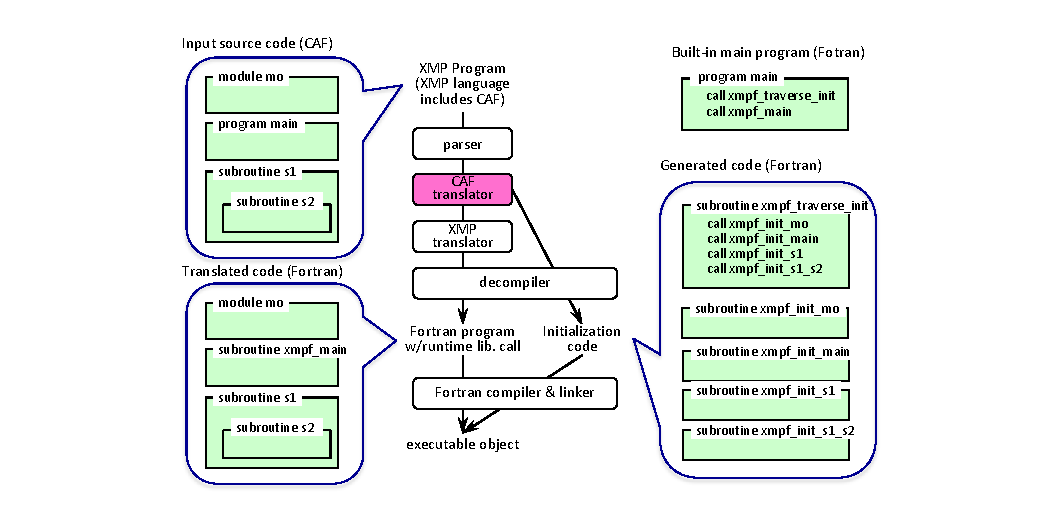
\includegraphics[scale=0.55,trim=6cm 0cm 4cm 6cm,clip]{figs/translator-tmp.pdf}
  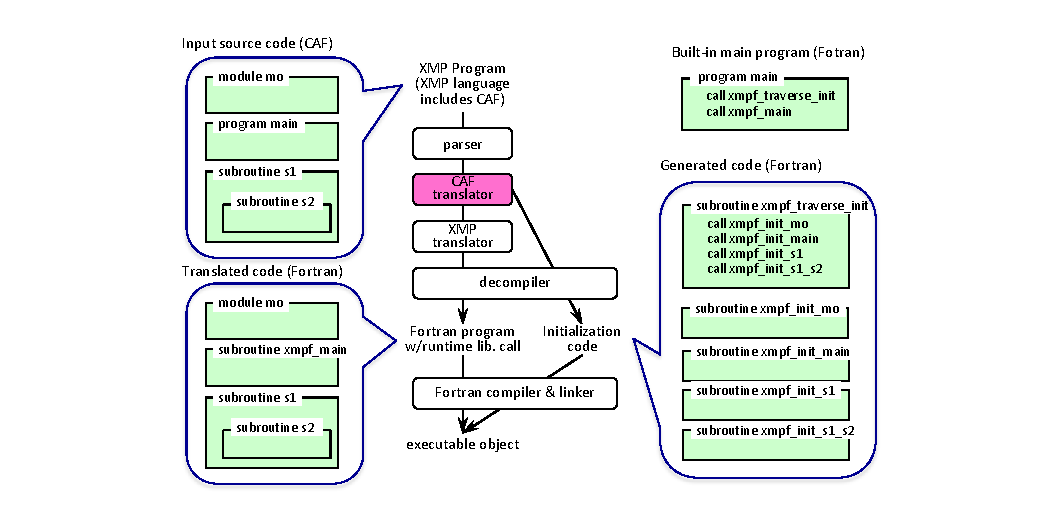
\includegraphics[trim=30mm 0mm 20mm 7mm, scale=1.0]{figs/translator-tmp.pdf}
  \caption{XMP compiler and an example of coarray program compilation}
  \label{fig:translator}
  %-- 修正すべき箇所
  CAF translator $\rightarrow$ coarray translator
 \end{center}
\end{figure}


%-----------------------------------------------------------------------------
\subsection{Allocation and Registration}
%-----------------------------------------------------------------------------

To be accessed using the underlying communication library,
the allocated coarray data must be registered to the library.
The registration contains all actions to allow the data to be accessed 
from the other nodes, including pin-down memory, acquirement of the global address,
and sharing information among all nodes.

%===========================================================
\subsubsection{Three methods of memory management}
%===========================================================

The coarray translator and the runtime library implements three methods of
memory management.
\begin{itemize}
\item
The {\bf Runtime Sharing (RS) Method} allocates and registers a large memory 
for all static and dynamic coarrays at the initialization phase.
The registered memory is shared by all static and allocatable coarrays. 

\item
The {\bf Runtime Allocation (RA) Method} allocates and registers a large memory
for all static coarrays at the initialization phase.
And it allocates and registers each allocatable coarray at runtime.

\item
The {\bf Compiler Allocation (CA) Method} allocates all coarray objects by 
the Fortran system (at compile time or at runtime) and the address is 
passed to the runtime library to be registered.
\end{itemize}

For the RS and RA methods, 
because the allocated memory address is determined in the runtime library, 
the object code must accept the address allocated 
inside the runtime system as an address of a regal Fortran variable.
To make this connection, it was necessary to use the Cray pointer, which is not 
in the Fortran standard.
In the case of the CA method, the runtime library accepts the address allocated
in the Fortran system, and registers to the communication library.

%
% 3 methodsの比較表を載せるならここか
%


%===========================================================
\subsection{Initial Allocation}
%===========================================================

Static coarrays are allocated and registered in the initializaton subroutines 
{\tt xmpf\_init\_{\it foo}}. 

On the {\bf Runtime-library Sharing (RS) method} and 
on the {\bf Runtime-library Allocation (RA) method},
static coarrays are initialized before the execution of the user program,
as follows.
\begin{itemize}
\item
In the first pass, all sizes of static (non-allocatable) coarrays are summed.
The size of each static coarray is evaluated form the declaration 
statement of each coarray. Because the dimensions may have any 
integer constant expression, the coarray translator 
evaluates name of constants, binary and unary operations, and 
basic Fortran intrinsic functions such as min/max and sum.
\item
Then, the total size of static coarrays is allocated and the address
and the size is registered to the underlying communication library.
\item
In the second pass, the addresses of the all coarrays are calculated to share
the registered data.
Due to the language specification, sizes of the same coarray are the same 
among all images (nodes). So the offset from the base address of the registered 
data for each coarray can be the same among all images.
\end{itemize}

In the RS method, allocatable coarrays are also shared the registered memory. 
The total size of the memory to be registered
should be specified with an environment variable by the user.
While in the RA method, the total size is fully calculated by the runtime 
library and no information is required to the user because allocatable coarrays
will be dynamically allocated on the other memories.

On the {\bf Compiler Allocation (CA) method},
the Fortran processor allocates each coarray and then the runtime library
registers the address.
Each static coarray is converted into a common (external) variable to share 
between the user-defined procedure (say {\it foo}) and its initialization
procedure ({\tt xmpf\_init\_{\it foo}}). The data is statically allocated
by the Fortran system similarly to the usual common variable.
the address is registered in the initialization procedure via the runtime
library.


%===========================================================
\subsubsection{Allocation at Runtime}
%===========================================================

For the RS method, the runtime library has a memory management system for
cutting out and retrieving memory for each allocation and deallocation of 
coarrays.

Figure~\ref{fig:register-RA-CA} illustrates the memory allocation and registration
for allocatable coarrays on the RA and CA methods. 

\begin{figure}[tbh]
 \begin{center}
  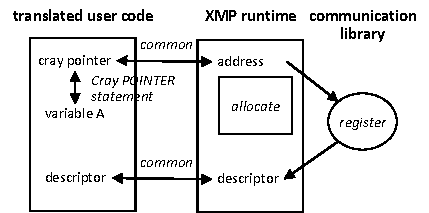
\includegraphics[scale=0.9, trim=0mm 0mm 0mm 0mm, clip]{figs/register-RA-tmp.pdf}\\
The runtime allocates and registers coarrays and passes the address to the user code.
 \end{center}
 \begin{center}
(a) RA method
 \end{center}
 \begin{center}
  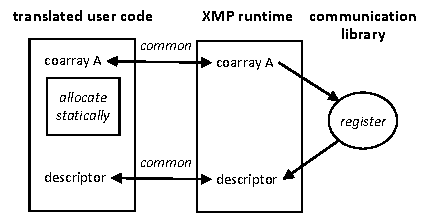
\includegraphics[scale=0.9, trim=0mm 0mm 0mm 0mm, clip]{figs/register-CA-tmp.pdf}\\
The user code allocates coarrays and causes the runtime to register with the address.
 \end{center}
 \begin{center}
(b) CA method
 \end{center}
 \caption{Memory allocation for coarrays in RA and CA methods}
 \label{fig:register-RA-CA}
\end{figure}

These methods are properly used by the underlying communication library.
%
On GASNet, only the RS method is adopted because its allocation function
can be used only once in the program.
%
On MPI-3, the CA method is not suitable because frequent 
allocation and deallocation of coarrays cause expensive creation and freeing 
MPI windows.
%
Over FJ-RDMA, the RS method has no advantage over the other methods.
Since the allocated address is used for registration to FJ-RDMA, 
no advantage was found for managing memory outside of the Fortran system. 
The unusual connection through the Cray pointer causes the degrade of 
the Fortran compiler optimization.


%-----------------------------------------------------------------------------
\subsection{PUT/GET Communication}\label{sec:putget}
%-----------------------------------------------------------------------------

To avoid disturbing the execution on the remote image, PUT and GET communications
are implemented always using Remote Direct Memory Access (RDMA) provided by 
the communication library (except coarrays with pointer/allocatable structure components). 
In contrast, local data access is selective between using Direct Memory Access (DMA) or
using a local buffer. For the buffer scheme, one of four algorithms will be chosen 
depending on three parameters, the size of the local buffer $B$ and the 
local and remote contiguous lengths $N_L$ and $N_R$.
$B$ should be large enough to ignore communication latency overhead and we use
about 400 kilo-bites in default. Unlike the case of MPI message passing,
coarray PUT/GET communication requires only one local buffer for any numbers of
other images.
$N_L$ and $N_R$ can be evaluated at runtime. The Fortran syntax guarantees 
that $N_L$ is a multiple of $N_R$ or $N_R$ is a multiple of $N_L$.
An algorithm to get the contiguous length is shown in the paper~\cite{pgas15}.

\tab{putget} summarizes our algorithm for PUT/GET communication for five cases.
The unit size is the chunk length of the PUT/GET communication.
Case~0 shows the algorithm using RDMA-DMA PUT/GET communication and Cases~1 through~4
shows the algorithms using RDMA and local-buffering. 
Due to its strict condition, the DMA scheme is rarely used.
And it is not always faster than the buffering scheme cases~2 and~3 because of the 
difference of the unit sizes. The merit of cases~2 and~3 is that the unit size 
is extended to a multiple of $N_L$ by gathering number of short contiguous data in the buffer,
or by scattering from the buffer into number of short contiguous data.

\begin{table}[tbh]
 \caption{Summary of the PUT/GET algorithm related to $N_L$, $N_R$ and $B$}
 \label{tab:putget}
 \begin{flushleft}
  \begin{tabular}{|@{~}c@{~}|c||@{~}c@{~}|@{~}c@{~}|}
\hline
scheme &
case &
condition &
unit size \\
\hline
\hline
DMA &
&
Local data is registered. &
$\min(N_L, N_R)$ \\
\hline
buffering &
1 & 
$N_R \leq B,~ N_R \leq N_L$ &
$N_R$ \\
\cline{2-4}
&
2 &
$N_L < N_R \leq B$ &
$N_R$ \\
\cline{2-4}
&
3 &
$N_L < B < N_R$ &
multiple of $N_L$ ($\leq B$) \\
\cline{2-4}
&
4 &
$B < N_R,~ B \leq N_L$ &
$B$ (or less than $B$ at last) \\
\hline
  \end{tabular}
 \end{flushleft}
 \begin{flushleft}
  \begin{tabular}{|@{~}c@{~}|c||@{~~}l@{~~}|@{~~}l@{~~}|}
\hline
scheme &
case &
PUT action for every unit &
GET action for every unit \\
\hline
\hline
DMA &
&
put once &
get once \\
\hline
buffering &
1 &
buffer once and put once &
get once and unbuffer once \\
\cline{2-4}
&
2 &
buffer for each $N_L$, and put once &
get once, and unbuffer for each $N_L$ \\
\cline{2-4}
&
3 &
buffer for each $N_L$, and put once &
get once, and unbuffer for each $N_L$ \\
\cline{2-4}
&
4 &
buffer once and put once &
get once and unbuffer once \\
\hline
  \end{tabular}
 \end{flushleft}
\end{table}



%-----------------------------------------------------------------------------
\subsection{Non-blocking one-sided communication}
%-----------------------------------------------------------------------------

GET通信をできる限りnon-blockingとし、そして、その完了待ちを可能なら次のimage control statementまで遅延したい。
\fig{block-ex}に示したような、同じsegment内で同じリモートデータへ書いて読むような
ケースは大変まれで、殆どの場合には次のimage control statementまで遅延できる。
添字式やイメージ番号が定数でないことが多いので、コンパイル時の判定では遅い方に倒れてしまう。
まれなケースを除外するための実行時判定が望まれる。

正確な実行時判定を行うためには、現在non-blocking PUT通信中のcoarrayのアドレスのrangeと相手のimage番号を
ハッシュテーブルに記憶し、GET通信を行う前にそのrangeとimage番号に重なりがないことをチェックし、
重なりがあったらそこでPUT通信を完了させる、という方法が考えられる。
しかしこれでは、重なりが無い通常のケースでも重なりのチェックのコストが大きい。
コンパイラでの解析と動的なチェックを併用する、正確さが劣ってもより高速な方法が望ましい。

現在の実装では、実行時の環境変数によってblockingとnon-blocking通信を選択する。
以下の条件に該当する場合には、低速となるblockingを選択しなければならない。
 明示的な同期なしで、リモートのcoarray変数に対して定義後の参照がある。




%\cleardoublepage

\section{Runtime Libraries}\label{sec:runtime}

%-----------------------------------------------------------------------------
\subsection{Layered Communication Libraries}
%-----------------------------------------------------------------------------

3種:one sided, collective, atomic. このうちcollectiveとatomicはMPIの機能をそのまま使う。
one sidedはallocate/freeとput/getと同期。
lower-level通信層のバリエーションを吸収するライブラリ層を設けた。階層の図。

\begin{figure}[tbh]
  \begin{center}
    % trimはleft bottom right topの順
    \fbox{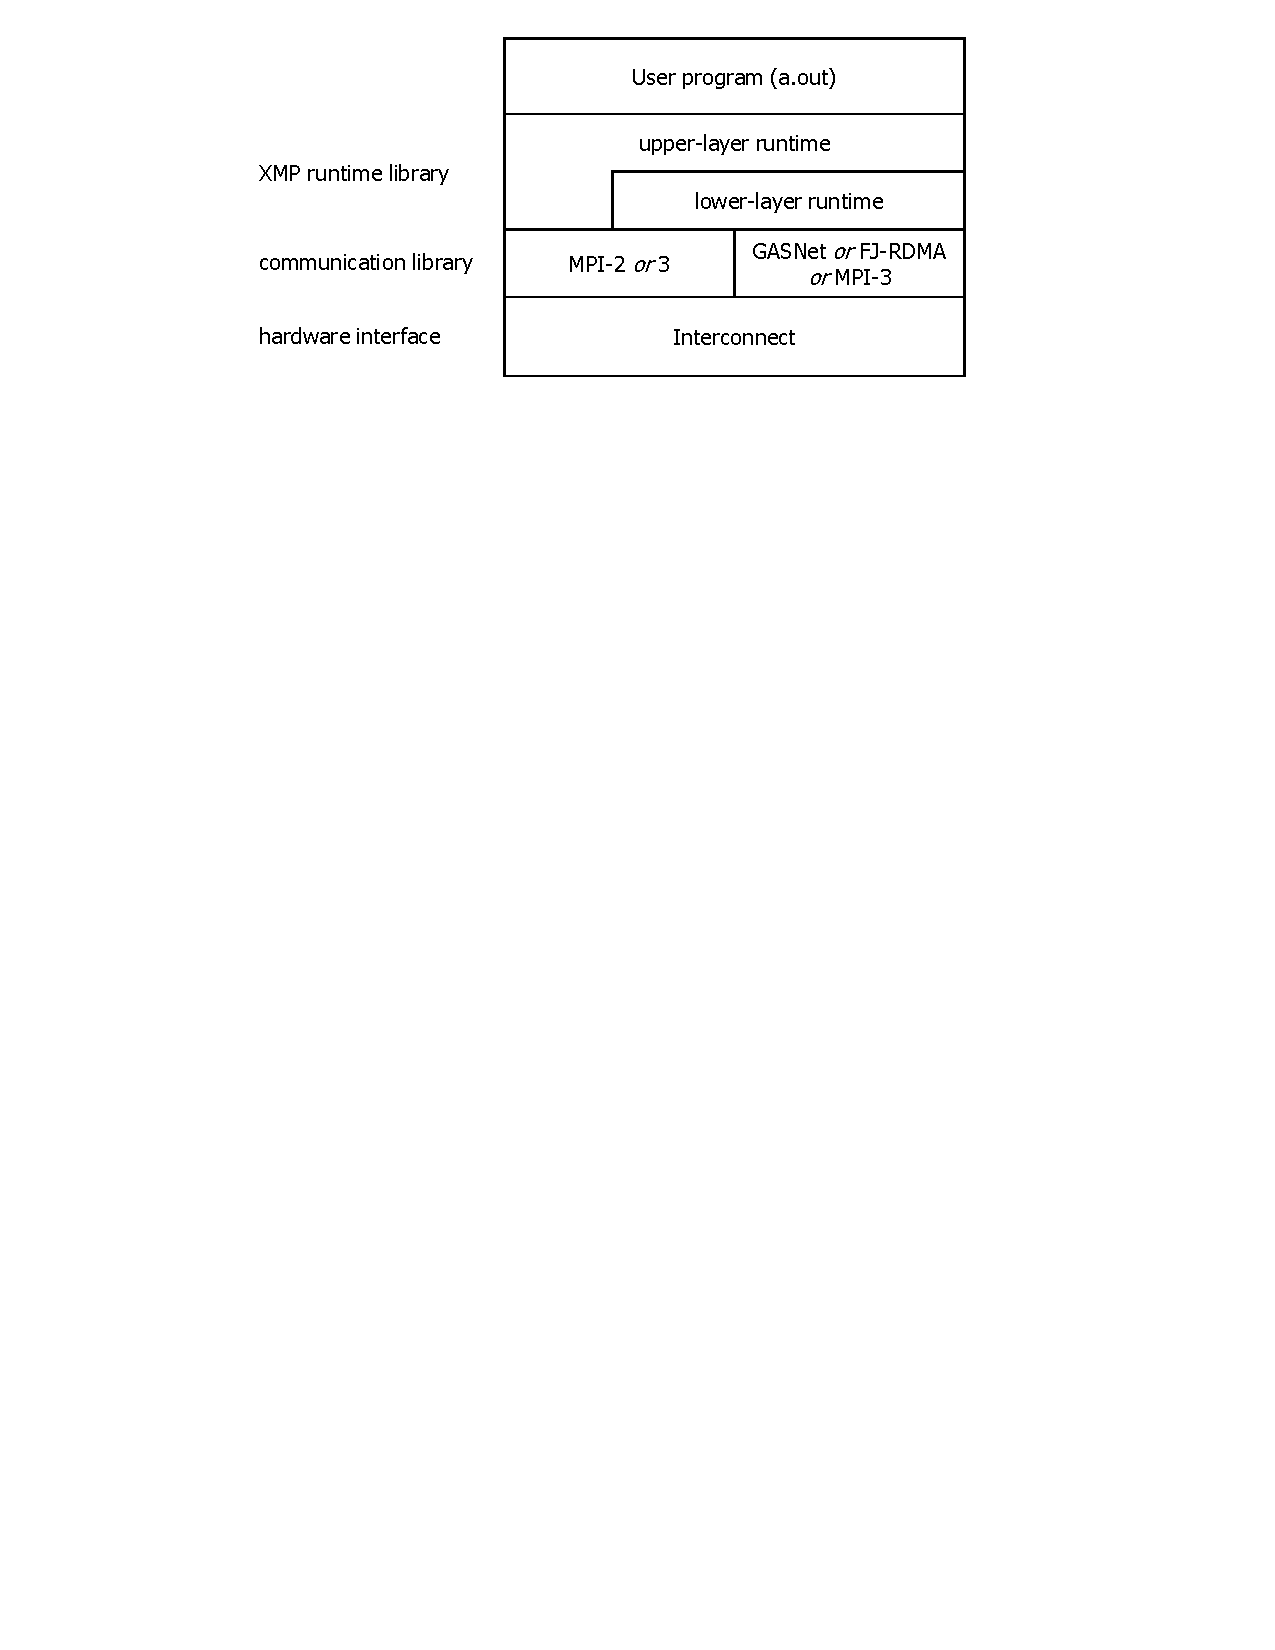
\includegraphics[trim=42mm 210mm 47mm 0mm, scale=0.7,clip]{figs/softstack.pdf}}
    \caption{Software stack for coarray features}\label{fig:layer}
  \end{center}
\end{figure}


To implement one-sided communication, the XcalableMP (XMP) runtime library selects one of the 
{\bf communication libraries}, MPI-3, GASNet, or Fujitsu’s native interface FJ-RDMA, 
as specified at build time. All coarray data must be {\bf registered} to the communication 
library to be referenced or defined via the communication library.

MPI-3 can be selected for all platform on which MPI-3 is implemented. Coarrays are 
registered and deregistered at the start and end point of the MPI window. 
Coarrays are performed one-sided communication by {\tt MPI\_Put} and {\tt MPI\_Get}, 
and synchronized by {\tt MPI\_Win\_fence}. 
Implementation on MPI incurs certain costs for dynamic allocation of coarrays and 
waiting for communication completion.

GASNet can be selected for more advanced implementation over InfiniBand. 
Since allocation and registration of are inseparable and can be done only once 
on GASNet, the implementation allocates and registers a huge pool at the startup 
of program execution to contain all coarray variables. 
The XMP runtime should allocate and deallocate coarrays not using the Fortran 
library but using the memory manager made for the pool.

FJ-RDMA can be selected for the implementation over Tofu interconnect of the K computer 
and Fujitsu PRIMEHPC FX10 and FX100. Basically, each coarray is allocated by the Fortran 
library and registered with {\tt FJMPI\_Rdma\_reg\_mem}. And it is deregistered with 
{\tt FJMPI\_Rdma\_dereg\_mem} before deallocated by the Fortran library. 
One-sided communication is performed with {\tt FJMPI\_Rdma\_put} and {\tt FJMPI\_Rdma\_get}, 
which include confirmation of communication completion.


\subsection{Intermediate Communication Library Interface}

サイトの内容に直す




次元の概念とcontiguityを上位層で解決するため結果的に必要なインタフェースは少なくなった。表

\begin{table}
 \begin{center}
  \caption{使用したCoarrayランタイムインタフェース(未公開機能関連を除く)}
  \begin{tabular}{|l|l|}
\hline
割付け・解放と登録
& 1. \verb|_XMP_coarray_malloc_image_info_1|\\
& 2. \verb|_XMP_coarray_malloc_info_1|\\
& 3. \verb|_XMP_coarray_malloc_do|\\
& 4. \verb|_XMP_coarray_regmem_do|\\
& 5. \verb|_XMP_coarray_lastly_deallocate|\\
\hline
片側通信
& 6. \verb|_XMP_coarray_shortcut_get|\\
& 7. \verb|_XMP_coarray_shortcut_put|\\
\hline
同期
& 8. \verb|xmp_sync_all|\\
& 9. \verb|xmp_sync_image|\\
& 10 \verb|.xmp_sync_images|\\
& 11 \verb|.xmp_sync_images_all|\\
& 12 \verb|.xmp_sync_memory|\\
\hline
atomic通信
& 13 \verb|._XMP_atomic_define_0|\\
& 14 \verb|._XMP_atomic_define_1|\\
& 15 \verb|._XMP_atomic_ref_0|\\
& 16 \verb|._XMP_atomic_ref_1|\\
\hline
問合せ
& 17 \verb|.xmp_all_num_nodes|\\
\hline
エラー処理
& 18 \verb|._XMP_fatal|\\
\hline
  \end{tabular}
 \end{center}
\end{table}


下位通信層は通信ライブラリを隠蔽する。例えばregisterは

しかしあらわになるものがあってオブジェクトが通信ライブラリを意識するモードで分ける。


%\cleardoublepage

\section{Evaluation}\label{sec:eval}

\subsection{Aggregated Nonblocking Communication}


\begin{figure}[tbh]
  \begin{center}
  % trimはleft bottom right topの順
  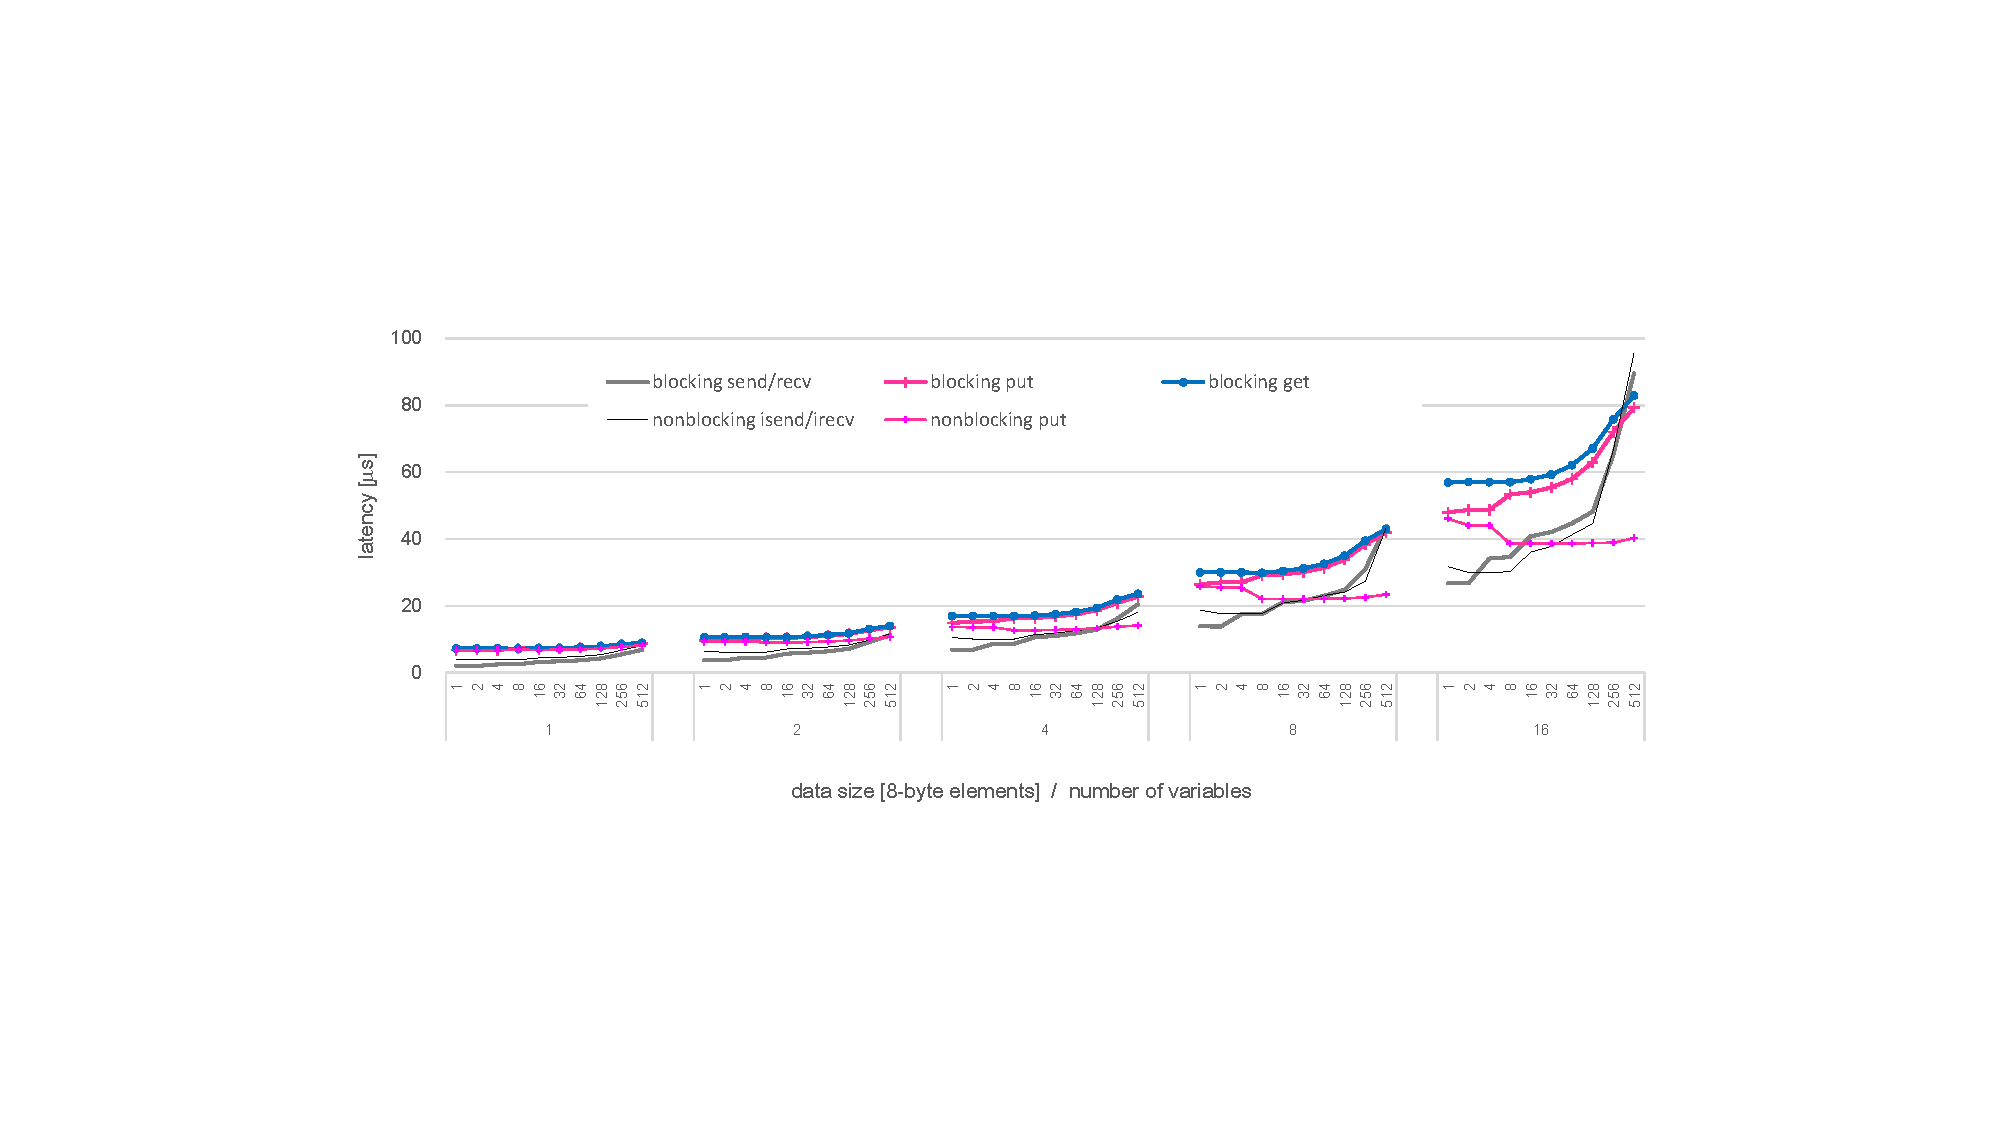
\includegraphics[scale=0.55,trim=6cm 0cm 4cm 6cm,clip]{figs/latency-16var.pdf}

  latency-16var.pdf\\
  2からの4つにして図を大きくする。
  \caption{n-var latency of pingpong}\label{fig:nvar-pp}
  \end{center}
\end{figure}

n-varの効果があった。実際のアプリでもこれはよく起こるパターンである。


\begin{figure}[tbh]
  \begin{center}
  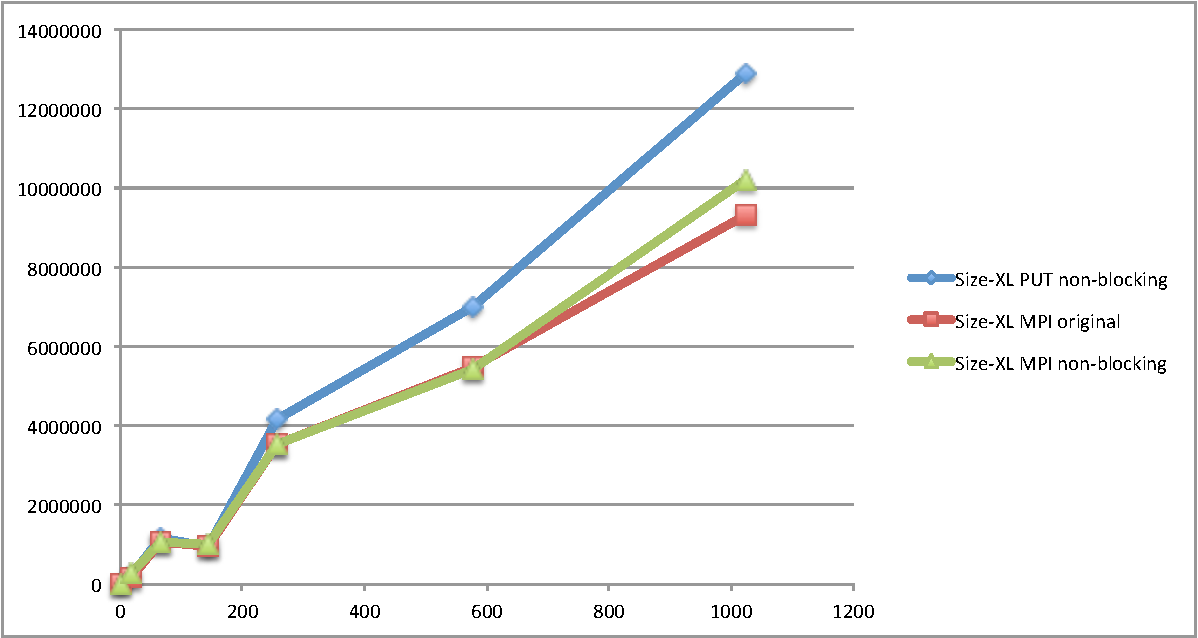
\includegraphics[scale=0.55]{figs/himeno.pdf}

  棒グラフにしてLを加えて2つにするかMまで加えて3つにする

  cf.\ air:/Users/iwashita/Desktop/coarray/Project\_Coarray/coarray\_runtime.pdf

  \caption{Himeno XL}\label{fig:himeno}
  \end{center}
\end{figure}


どういうパターンか分析して説明。n個のcontiguousなnonblocking comm.


%\cleardoublepage

\section{Related Work}\label{sec:related}

%-- Coarray Imprementations
The Universicy of Rice has implemented coarray features with their own extension called CAF~2.0.
It is a source-to-source compiler based on the ROSE compiler. GASNet is used as its 
communication layer.
%
Houston University depeloped UH-CAF onto the Open64-base OpenUH compiler. It supports
coarray features defined in the Fortran 2008 standard. As the communication layer,
GASNet and ARMCI can be used selectively.
%
OpenCoarrays~\cite{OpenCo} is an open-source software project. It is an library 
which can be used with GNU Fortran (gfortran) V5.1 or later. It supports coarray features
specified in Fortran 2008 and a part of Fortran 2018.  As the communiation layer,
MPICH and GASNet can be used selectively.
%
In the vendors, Cray and Intel fully and Fujitsu partially support the coarray features
specified in Fortran 2008.


task間はF2018のcoarrayにある。違いは・・・

getのnonblockingは難しい。書式上、獲得したあたいがすぐに使用されることになるため、
nonblockingのrangeを大きく取れない。
putでは完了を遅延させるのにたいし、開始を先行させる技術(prefetching)が考えられる。
Crayはそのためのdirectiveをもつ。

RiceもCrayポインタを使っている。
Crayポインタはalias analysisで性能を落とす。


\section{Future Works}\label{sec:related}

Coarray C++はObject oriented programmingになれた人には自然な実装と感じるかもしれない。
我々の目指すCoarray Cはこれとは違い、HPCプログラムをCで書いている人向けに修正を最小限
にするものである。また、coarrayを抽象性の高い概念で定義するのではなく、
単にアドレスと長さで特定できるメモリの範囲と定義したい。これによって一般の
Cプログラマがキャストや引数渡しを使って同じ領域を目的によって連続配列や多次元配列
や単に先頭アドレスへのvoidポインタなどとして自由に使い回すように扱いたい。
これは美しくはないが、Cの大きなプログラムを抱えている利用者には必要である。
仕様書の定義には曖昧さが残っているので、まだ修正が必要である。
Fortranと同じような性能が出せるもので、かつ、FortranのCoarrayとの互換性を持たせたい。

Non-blocking PUT communication 
正確な実行時判定を行うためには、現在non-blocking PUT通信中のcoarrayのアドレスのrangeと相手のimage番号を
ハッシュテーブルに記憶し、GET通信を行う前にそのrangeとimage番号に重なりがないことをチェックし、
重なりがあったらそこでPUT通信を完了させる、という方法が考えられる。
しかしこれでは、重なりが無い通常のケースでも重なりのチェックのコストが大きい。
コンパイラでの解析と動的なチェックを併用する、正確さが劣ってもより高速な方法が望ましい。


%\cleardoublepage

\section{Conclusion}\label{sec:concl}


%\cleardoublepage

\appendix

\section{MEMO}
MPIはPGASに向かない、という論文がどこかに。

\section{Fusen}
\begin{verbatim}

synmetric memory
リモートのアドレスをローカルで計算できる
これがあるから、片側通信が。。。


下位層:通信libの差異を吸収し、上位層にプリミティブを提供する。
XMP coarray実装のプリミティブi/f
put operation
get operation
- どちらも連続データのみ/nonblocking。
sync memory operation
- 発行したputをすべてremoteに書き込み、getをすべてlocalに読み込むまで待つ。

putにはnonblocking技術:runtimeで十分
getにはprefetch技術:コンパイラ技術


生産性の観点の評価
1. リンク時にstatic配列を集めるところが対MPI片側通信で重要。言語仕様/言語処理系だからできる。単にライブラリ群/ライブラリ呼出しではできない。
2. F90配列記述がMPI_Typeの定義を不要にしている。


klogin7$ which xmpf90
~/Project/OMNI-clone/bin/xmpf90
klogin7$ xmpf90 --version
Version:1.3.1, Git Hash:4a5736e
klogin7$ 


sync memoryがいつ必要か
- ユーザ記述
- getのとき、1subarray参照に対してsyncmemoryを1回にする。
- getの前に、同じremoteアドレスへのputがあればsyncmemoryで待つ


alignmentの問題か
64バイト未満でputのlatencyが高い。
src5, RUN5で改善 ・・・しなかった
メモリ割付けのalignmentの問題ではない。
残るはTofuのputの単位の問題と推測
マスク付き書き込みになる?
この点ではRDMAよりバッファリングが有利


A Source-to-Source Translation of Coarray Fortran with MPI for High Performance
https://dl.acm.org/citation.cfm?id=3155888&dl=ACM&coll=DL

Preliminary Implementation of
Coarray Fortran Translator Based on Omni XcalableMP
https://ieeexplore.ieee.org/document/7306099

\end{verbatim}


\section{STATUS-CAF}
\begin{verbatim}

1.2  Interoperability with the global-view features (NEW since V1.0)
  Coarray features can be used inside the TASK directive blocks. As default,
  each coarray image is mapped one-to-one to a node of the current executing 
  task. I.e., num_images() returns the number of nodes of the current executing 
  task and this_image() returns each image index in the task.
     There are two directives to change the default rule above. A COARRAY 
  directive corresponding to a coarray declaration changes the image index set 
  of the specified coarray with the one of the specified nodes. An IMAGE 
  directive corresponding to one of a SYNC ALL statement, a SYNC IMAGES 
  statement, a call statement calling CO_SUM, CO_MAX, CO_MIN or CO_BROADCAST 
  changes the current image index set with the one of the specified nodes.
  See the language spacifications [3].

2. Declaration
  Either static or allocatable coarray data objects can be used in the program. 
  Use- and host-associations are available but common- or equivalence-
  association are not allowed in conformity with the Fortran2008 standard.
  Current restrictions against Fortran2008 coarray features:
    * Rank (number of dimensions) of an array may not be more than 7.
    * A coarray cannot be of a derived type nor be a structure component.
    * A coarray cannot be of quadruple precision, i.e., 16-byte real or 32-byte 
      complex.
    * Interface block cannot contains any specification of coarrays. To describe
      explicit interface, host-assocication (with internal procedure) and use-
      association (with module) can be used instead.
    * A pointer component of a derived-type coarray is not allowed.
    * An allocatable component of a derived-type coarray cannnot be referrenced
      as a coindexed object.
    * A derived-type coarray cannot be defined as allocatable.
      
2.1  Static Coarray
  E.g.
      real(8) :: a(100,100)[*], s(1000)[2,2,*]
      integer, save :: n[*], m(3)[4,*]
  The data object is allocated previously before the execution of the user 
  program.  A recursive procedure cannot have a non-allocatable coarray without 
  SAVE attribute.
  Current restrictions against Fortran2008 coarray features:
    * Each lower/upper bound of the shape must be such a simple expression that 
      is an integer constant literal, a simple integer constant expression, or
      a reference of an integer named constant defined with a simple integer 
      constant expression.
    * A coarray cannot be initialized with initialization or with a DATA 
      statement.
    
2.2  Allocatable Coarray
  E.g.
      real(8), allocatable :: a(:,:)[:], s(:)[:]
      integer, allocatable, save :: n[:], m(:)[:,:]
  The data object is allocated with an ALLOCATE statement as follows:
      allocate ( a(100,100)[*], s(1000)[2,2,*] )
  The allocated coarray is deallocated with an explicit DEALLOCATE statement or 
  with an automatic deallocation at the end of the scope of the name unless it 
  has SAVE attribute.
  Current restrictions against fortran2008 coarray features:
    * A scalar coarray cannot be allocatable.
    * An allocatable coarray as a dummy argument cannot be allocated or 
      deallocated inside the procedure.
    
3. Reference and definition of the remote coarrays
  For the performance of communication, it is recommended to use array 
  assignment statements and array expressions of coindexed objects as follows:
      a(:) = b(i,:)[k1] * c(:,j)[k2]    !! getting data from images k1 and k2
      if (this_image(1))  d[k3] = e     !! putting data d on k3 from e
  Current restrictions on the K computer and Fujitsu PRIMEHPC FX10:
    * The coindexed object/variable must be aligned with the 4-byte boundary 
      and the size of the array elements of them must be a multiple of 4 bytes.
  
4. Image control statements
  SYNC ALL, SYNC MEMORY and SYNC IMAGES statements are available.
  Current restrictions against Fortran2008 coarray features:
    * LOCK, UNLOCK, CRITICAL and END CRITICAL statements are not supported.
    * STAT= and ERRMSG= specifiers of image control statements are not 
      supported.
    * ERROR STOP statement is not supported.
    
5. Incrinsic Functions
  Inquire functions NUM_IMAGES, THIS_IMAGE, IMAGE_INDEX, LCOBOUND and LUBOUND
  are supported.
  Current restrictions against Fortran2008 coarray features:
    * ATOMIC_DEFINE and ATOMIC_REF subroutines are not supported.

6. Intrinsic Procedures in Fortran2015
  Argument SOURCE can be a coarray or a non-coarray.
  Intrinsic subroutines CO_BROADCAST, CO_SUM, CO_MAX and CO_MIN can be used 
  only in the following form:
    * CO_BROADCAST with two arguments SOURCE and SOURCE_IMAGE
      E.g.,  call co_broadcast(a(:), image)
    * CO_SUM, CO_MAX and CO_MIN with two arguments SOURCE and RESULT
      E.g.,  call co_max(a, amax)



\end{verbatim}


\section{mac-air memo}
\begin{verbatim}

introduction
coarrays in XcalableMP
support F2008 coarrays
image setをtaskに対してmap
natural extension to C
basic implementation and issues
lower-level interface
evaluation
related work
Coarray C++は
task間はF2018のcoarrayにある。違いは・・・
Crayはgetをdirectiveで実装
conclusion

implementation for high performance
static coarrayの高速化
全部まとめて先にallocするコンパイラ技術
定数評価、構造体の大きめな見積り
allocatable coarrayの高速化:lowlevelに合わせて選択
RuntimeLibShare事前に巨大領域を取る
実行時allocのコストが大きいとき
RuntimeLibAllocation実行時allocのコストが小さいとき
contiguouity検出による高速化
次元を跨ぐ連続性抽出
バッファリング
有限サイズ、基礎データから、Nlocal, Nremote, Nbufの関係でアルゴリズム
CommpilerAllocationFortranがallocateしてregisterできるとき

implementation software layer
3種:one sided, collective, atomic. このうちcollectiveとatomicはMPIの機能をそのまま使う。それ以上の工夫はない。one sidedはallocate/freeとput/getと同期。lower-level通信層のバリエーションを吸収するライブラリ層を設けた。階層の図。
次元の概念とcontiguityを上位層で解決するため結果的に必要なインタフェースは少なくなった



\end{verbatim}


\section{nigun}
\subsection{introよりrelated workの方がよいか?}



PGAS言語の一つであるCoarray Fortran(CAF)は,Fortran 2008仕様の一部として採用されたことも追い風となって,近年研究開発が盛んに進められている.フリーのものでは, Houston大学のOpenUHコンパイラを開発基盤としたUH-CAF[5]と,Rice大学のROSEコンパイラを開発基盤としたcaft[6]が有名である.近年リリースされたOpenCoarrayは,GNU gfortranにリンクできるライブラリである.我々の開発するOmni XMPもまた,CAFコンパイラとして利用することができる.ベンダではCrayとIntelが古くから提供しており,近年富士通からもリリースされている.これら3社は,Fortran 2008と2015に含まれるcoarray機能の実装をFortran2003のフル実装よりも先行させたことになる.
Omni XMPは,PCクラスタコンソーシアムのXcalableMP規格部会が制定する並列言語XcalableMP(XMP)のパイロット実装である.XMPは,FortranとCをベースとし,ディレクティブ行の挿入によって並列化を記述するが,Fortran 2008で定義されるcoarray機能も仕様として含んでいる.前者は「逐次プログラムに指示を与えて並列化する」という考え方からグローバルビューと呼ばれ,並列プログラミングが容易にできることを狙う.後者は「個々のノード(イメージ)の挙動を記述する」という考え方でローカルビューと呼ばれ,MPIに匹敵する性能がMPIよりも容易に出せることを狙っている.




                                   
\begin{thebibliography}{99}
\addcontentsline{toc}{chapter}{\bibname}
 \bibitem{xmp} XcalableMP Language Specification, \url{http://xcalablemp.org/specification.html} (2017).
 \bibitem{openacc} The OpenACC Application Programming Interface, \url{http://www.openacc.org} (2015).
 \bibitem{mpi} MPI: A Message-Passing Interface Standard, \url{http://mpi-forum.org} (2015).
 \bibitem{coarray} John Reid, JKR Associates, UK. Coarrays in the next Fortran Standard.
    ISO/IEC JTC1/SC22/WG5 N1824, April 21, 2010.
 \bibitem{coarray18} ISO/IEC TS 18508:2015, Information technology -- Additional Parallel 
    Features in Fortran, Technical Specification, December 1, 2015.
 \bibitem{F08} Fortran~2008
 \bibitem{F18} Fortran~2018

 \bibitem{Rice}
 \bibitem{HU}
 \bibitem{OpenCo} http://www.opencoarrays.org/

\end{thebibliography}

\end{document}



